7.	如图,将一个圆盘6等分,写出指针落在下列区域的可能性大小:

\begin{center}

    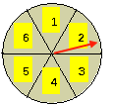
\includegraphics[height=3cm]{lib/image/MJA03060107.png}

\end{center}

\begin{subquestions}

    \subquestion 指针落在4的可能性大小是\key{\hspace{2cm}};

    \subquestion 指针落在奇数区域的可能性大小是\key{\hspace{2cm}};

    \subquestion 指针落在合数区域的可能性大小是\key{\hspace{2cm}}.    

\end{subquestions}



